    \documentclass{article}
% \usepackage[spanish]{babel}
% \usepackage[9pt]{extsizes}
\usepackage[T1]{fontenc}
\usepackage[spanish,mexico]{babel}
\usepackage[utf8]{inputenc}
\usepackage[margin=1cm,top=2cm,bottom=2cm,a4paper]{geometry}
\usepackage{amsmath}
\usepackage{amssymb}
\usepackage{bm}
\usepackage{graphicx}

\usepackage{mdframed}
\newmdtheoremenv[outerlinewidth=3,leftmargin=-8pt,%
rightmargin=-12pt,backgroundcolor=white,%
outerlinecolor=blue,innertopmargin=1pt,
% innerrightmargin=3pt,%
splittopskip=\topskip,ntheorem, font = {\sffamily}]{formuleo}%
{Ecuaciones}



\newcommand{\tita}{\theta}
\newcommand{\substy}[2]{\ensuremath{{#1_{\mathrm{#2}}}}}
\newcommand{\sib}[1]{\ensuremath{\left[\si{#1}\right]}}
\newcommand{\degree}{\ensuremath{{^\circ}}}
\newcommand{\attackangle}{{\ensuremath{\bm{\alpha}}}}
\newcommand{\cp}{{c_p}}
\newcommand{\cv}{{c_v}}
\newcommand{\cteuniversal}{\ensuremath{\tilde{R}}}
\newcommand{\molarmass}{\ensuremath{{\scriptstyle \bar{M}}}}
\newcommand{\Rconst}{R}
\newcommand{\gasconst}{k}
\newcommand{\ctegas}{\gasconst}
% \newcommand{\speedsound}{{c_{\!s\!}}}
\newcommand{\relative}{\mathrm{rel}}
\newcommand{\speedsound}{a}
\newcommand{\ctan}[1]{\ensuremath{c_{\theta #1}}}
\newcommand{\crad}[1]{\ensuremath{c_{r #1}}}
\newcommand{\cax}[1]{\ensuremath{c_{a #1}}}
\newcommand{\angvel}{\ensuremath{\omega}}
\newcommand{\Mach}{\mathrm{M}}
\newcommand{\di}{\textrm{d}}
\newcommand{\cte}{\textrm{cte}}
%Entradas para glosario 
\newcommand{\etaiso}{\eta_{\mathrm{iso}}}
\newcommand{\etaint}{\eta_{\mathrm{int}}}
% \newcommand{\etamec}{\eta_{\mathrm{mec}}}
\newcommand{\Sgen}{\substy{S}{gen}}
\newcommand{\dQ}{\dot{Q}}
\newcommand{\dW}{\dot{W}}
\newcommand{\dm}{\dot{m}}
\newcommand{\etaTot}{\substy{\eta}{iso}}
\newcommand{\etahid}{\substy{\eta}{h}}
\newcommand{\etamec}{\substy{\eta}{m}}
\newcommand{\etavol}{\substy{\eta}{vol}}
\newcommand{\slip}{\xi}
\newcommand{\slipangle}{\ensuremath{\theta_d}}
\newcommand{\radrel}{\nu}
\newcommand{\rext}{\substy{r}{ext}}
\newcommand{\rbase}{\substy{r}{base}}
\newcommand{\powerreduction}{\mu}
\newcommand{\degreeofreaction}{{\bm{R}}}
\newcommand{\relcomp}{{\ensuremath{r_{\!c}}}}
\newcommand{\epsi}{\varepsilon}
\newcommand{\dV}{\dot{V}}
\newcommand{\dv}{\dot{v}}
\newcommand{\adim}[1]{\ensuremath{\mathrm{#1}}}
\newcommand{\Nusselt}{\adim{Nu}}
\newcommand{\Reynolds}{\adim{Re}}
\newcommand{\Grashof}{\adim{Gr}}
\newcommand{\Prandtl}{\adim{Pr}}
\newcommand{\Biot}{\adim{Bi}}
\newcommand{\Fourier}{\adim{Fo}}
\newcommand{\crit}{\mathrm{crit}}
\newcommand{\going}{\ensuremath{\rightarrow}}
% \newcommand{\dQ}{\dot{Q}}
\newcommand{\starit}{\ensuremath{^{*}}}
\newcommand{\LMTD}{\operatorname{LMTD}}
\newcommand{\Stanton}{\adim{St}}
\newcommand{\separar}{\ensuremath{\pmb{  \parallel{} }}}
\newcommand{\entrada}{\mathrm{in}}
\newcommand{\out}{\mathrm{out}}
\begin{document}
\pagestyle{empty}
{
\centering
{\large Formuleo Turbomáquinas \par}

{\small Patricio Whittingslow --- 55423\par}
}
\fontsize{10}{0}
% \newcommand{\formuleoseparator}{\vfill}
\newcommand{\formuleoseparator}{}
\begin{formuleo}[Termodinámica]
Ecuaciones Cardinales: $T\di s = \di h - v \di p$ \separar $T\di s = \di u +p \di v$ \newline
\end{formuleo}

\formuleoseparator

\begin{formuleo}[Modelo gas ideal]
Gas Ideales: $\tilde{R}=8,314 $[J/mol/K]\separar $\tilde{R}=\molarmass R$, \molarmass [kg/mol]\separar $pV = m R T$ \separar $pv= RT$ \separar $pV = N\tilde{R}T$ \separar $a = \sqrt{Z_a \ctegas RT}$ \separar $T_{0}=T\left(1+\frac{k-1}{2} M^{2}\right)$ \separar $p_{0}=p\left(1+\frac{k-1}{2} M^{2}\right)^{\frac{k}{k-1}}$  \separar $\rho_{0}=\rho\left(1+\frac{k-1}{2} M^{2}\right)^{\frac{1}{k-1}}$ \\\newline

\textbf{Procesos incompresibles}: $s_{2}-s_{1}=\int_{T_{1}}^{T_{2}} \frac{\cv(T)}{T} d T$\newline
\textbf{Procesos compresibles isoentropicos:}
$\frac{T_{2}}{T_{1}}=\left(\frac{p_{2}}{p_{1}}\right)^{\frac{\ctegas-1}{\ctegas}}=\left(\frac{v_{1}}{v_{2}}\right)^{\ctegas-1}$ \separar $\left(\frac{T_{2}}{T_{1}}\right)^{\frac{\ctegas}{\ctegas-1}}=\frac{p_{2}}{p_{1}}=\left(\frac{v_{1}}{v_{2}}\right)^{\ctegas}$ \separar $\left(\frac{T_{1}}{T_{2}}\right)^{\frac{1}{\ctegas-1}}=\left(\frac{p_{1}}{p_{2}}\right)^{\frac{1}{\ctegas}}=\frac{v_{2}}{v_{1}}$ \\
\textbf{Procesos compresibles isoentropicos:} $p_0=\cte=p+\frac{1}{2}\rho c^2$\separar $h_0=h+\frac{1}{2}c^2$ \\
\textbf{Gas perfecto:} $h=\cp T$;  $\cp = \ctegas R/(\ctegas -1)$ \going $T_0=T+\frac{1}{2}c^2/\cp $ \separar $s_{x}^{0}=s_{x}-s_{0}=\int_{T_{0}}^{T_{x}} \frac{c_{p}}{T} \mathrm{d} T \going s_{2}-s_{1}=c_{p} \ln \frac{T_{2}}{T_{1}}-R \ln \frac{p_{2}}{p_{1}}$


\end{formuleo}


\formuleoseparator
\begin{formuleo}[Fundamentales de turbomáquinas]
$\frac{\dW}{\dm} = U_1 \ctan{1} - U_2\ctan{2}= \left( \frac{w_2^2-w_1^2}{2} \right)+\left( \frac{c_1^2-c_2^2}{2} \right)+ \left( \frac{U_1^2-U_2^2}{2} \right)$ \separar 

$\eta_{t o b}=\frac{\text {Energía cinética actual de salida}}{\text {Energía cinética si el proceso fuera reversible}} =\frac{1-T_2/T_{01}}{1-T_{2s}/T_{01}}= \frac{\frac{1}{2} c_{2}^{2}}{\frac{1}{2} c_{2 s}^{2}}=K_{t o b}^{2}$ \separar $\eta_{d i f}=\frac{h_{2 s}-h_{1}}{h_{2}-h_{1}}=\frac{c_{1}^{2}-c_{2 S}^{2}}{c_{1}^{2}-c_{2}^{2}}=\frac{(p_2/p_1)^{(\ctegas-1)/\ctegas}-1}{\left[(p_{01}/p_{02})(p_2/p_1) \right]^{(\ctegas-1)/\ctegas}-1}$ \separar Grado de reacción: $\degreeofreaction=\frac{\text { Salto entálpico en rotor }}{\text { Salto entálpico total en etapa (rotor }+\text { estator } )} =\frac{\Delta h_{\mathrm{rotor}}}{\Delta h_{\mathrm{etapa}}}$\separar Maq. Hidraulicas: $ \degreeofreaction=\frac{p_{3}-p_{2}}{p_{3}-p_{1}}$ \separar   Pelton: $F_x=\rho A (c-u)^2(1-\cos \theta )$ \separar $\eta_{\mathrm{generadora}}=\frac{h_{02s}-h_{01}}{h_{02}-h_{01}}= \frac{\text{Trabajo adiabatico mínimo por seg.}}{\text{Trabajo adiabatico hecho por seg.}}$ \separar Turbinas: $\eta_{\mathrm{motora}}=\frac{h_{02}-h_{01}}{h_{02s}-h_{01}}$
\end{formuleo}

\formuleoseparator

\begin{formuleo}[Centrifugos] Adimensionalizacion dinámica: $\pi_{1}=\frac{p_{02}}{p_{01}}$, $\pi_{2}=\dot{m} \frac{\sqrt{R T_{01}}}{D^{2} P_{01}}$, $\pi_{3}=\frac{\Omega}{\sqrt{R T_{01}}}$, $\pi_{4}=\eta_{\mathrm{iso}}$\separar$\tan \beta_{1}=\frac{c_{a 1}}{U_{1}}$ \separar $\xi=\frac{c_{\theta d}}{c_{\theta}}=\frac{c_{\theta}-u_{d}}{c_{\theta}}$ \separar $D_{\mathrm{eddy}}\simeq \frac{\pi D_2\cos \beta_2}{Z}$ \separar $\frac{\dW_d}{\dm}=e_d = h_{02}-h_{01}=\ctan{2d} U_2 - \ctan{1} U_1 = (\slip \ctan{2})U_2 - \ctan{1} U_1$ 
\separar $\frac{p_{03}}{p_{01}}= \left( \frac{T_{03s}}{T_{01}}\right)^{\frac{\ctegas}{\ctegas-1}} =\left[ 1+ \frac{\etaiso (\slip \ctan{2}U_2 - \ctan{1}U_1)}{\cp T_{01}} \right]^{\frac{k}{k-1}}$ \separar $T_{03}-T_{01} = \frac{\xi \ctan{2} U_2 - \ctan{1}U_1}{c_p}$\separar $\Mach_1 = \frac{\cax{1}}{\speedsound} = \frac{\cax{1}}{\sqrt{\ctegas R T_1}}$ \separar $\Mach_2 = \frac{c_{2d}}{\sqrt{Z_2\ctegas R T_2}}$ \separar Coef. Lift: $\mathrm{C_L} = \frac{L}{\frac{1}{2} \rho c^2} bt$; $t$ es cuerda, $b$ es long. de perfil 
\end{formuleo}

\formuleoseparator

\begin{formuleo}[Axiales]
$\radrel = \frac{r_{\mathrm{ext}}}{r_{\mathrm{base}}}$ \separar $ \frac{\dW}{\dm} = U \cax{} (\cos\beta_2 - \cos\beta_1 )$ \separar Isoentropico: $h_3 - h_1 = \frac{p_3 -p_1}{\rho}=U (\ctan{3}-\ctan{1})$ \separar

$\powerreduction = \frac{\Delta \substy{T}{real}}{\Delta \substy{T}{euler}} \quad \text{tal que} \quad \substy{\dW}{real} = \powerreduction \dW$ \separar $\frac{p_{03}}{p_{01}} = \left[1 + \frac{\etaiso \powerreduction}{\cp T_{01}}U \cax{} (\tan \beta_1 - \tan \beta_2) \right]^{\frac{\ctegas}{\ctegas-1}}$ \separar $\degreeofreaction = \frac{h_2 - h_1}{h_3 - h_1}$ \going $\rho = \cte \Rightarrow \degreeofreaction = \frac{p_3}{p_1}$ 
\end{formuleo}

\formuleoseparator

\begin{formuleo}[Alternativos]
$\epsi_{vol}=1-C(\relcomp^{\frac{1}{n}} -1)=\frac{V_1 - V_4}{V_1 - V_3}$ \separar 
$\relcomp_{\max} = (1+C^{-1})^n$ \separar
$\epsi_{term}=T_{asp}/T_{int}$ \separar $\epsi_{pca}=\frac{P_{asp}}{P_{int}}$ \separar $ \epsi_{fugas} = \frac{1}{1+f}$ \separar$ \eta_{vol}=\prod_i^4 \epsi_i$ \separar $\dV = \pi r^2 L_{carr} f_{hz} X \etavol$ \separar $\dm = \frac{p \dV}{Z_e R}$ \separar $p_{int} = p_e \frac{A_p}{A_v}-\frac{kx}{A_v}-\Delta p$
\end{formuleo}
\formuleoseparator
\begin{formuleo}[Refrigeración]
Sin refrigeración: $\dW_{\mathrm{ad/rev}} = \dm \left[\frac{k}{k-1}R(T_{\out}-T_{\entrada}) \right]$ \separar 

Refrig. intermedia:$\dW_{\mathrm{pol/rev}}=\dm \left\{ \frac{n}{n-1} T_{\entrada} R \left[ \left(\frac{p_\out}{p_\entrada}\right)^{\frac{n-1}{n}} -1\right] \right\}$ \separar Refrig. máxima: $\dW_{\mathrm{isot/rev}}=\dm R T_\entrada \ln(\frac{p_\out}{p_\entrada})$
\end{formuleo}
\formuleoseparator
\begin{formuleo}[TdC]
Ecuación de calor: $\nabla^2T+\Dot{q_G}=\rho c \frac{\partial T}{\partial t}$ \separar
$q_k=-k\cdot A\frac{\Delta T}{\Delta x} $ \separar cilindricas: $q_k=2\pi Lk\frac{\Delta T}{\ln{\frac{r_o}{r_i}}}$ \separar esféricas: $q_k=\frac{\Delta T}{\left(\frac{r_o - r_i}{4\pi k r_o r_i}\right)}$ \separar Resistencias: $R_k=\frac{L}{kA}$, cilindro: $R_k=\frac{\ln{\frac{r_o}{r_i}}}{2\pi Lk}$, esfera: $R_k={\left(\frac{r_o - r_i}{4\pi k r_o r_i}\right)}$ \separar Aletas: $\eta=\frac{q}{q_{max}}=\frac{q}{hPL\Delta T_{b\infty}}$ \separar

$\alpha =\frac{k}{\rho c_p}$ \separar Modelo resistencia despreciable: $ \frac{\Delta T_{t\infty}}{\Delta T_{0\infty}}$=$e^{\Biot\Fourier}$ \separar Radiación: $q_r=\sigma T^4$ \separar$q_{r 1\leftarrow 2}=A_1 \mathcal{F}_{1,2} \sigma  T^4$;  $\mathcal{F}_{1,2}=f(\epsilon_2, \alpha_1 ,forma) $ \separar$\rho + \alpha + \epsilon =1$\separar Wien: $\lambda_{\max} T = 2,8976\times 10^{-3}$ \separar $r_{\mathrm{crit}}=\frac{k}{h}$
\end{formuleo}

\formuleoseparator


\formuleoseparator
\begin{formuleo}[Adimensionales]
 $\Reynolds=\frac{UL}{\nu}=\frac{\rho UL}{\mu}$\separar    $\Nusselt=\frac{\Bar{h}_c L}{k_{\mathrm{fluido}}}=\frac{\text{conveccion}}{\text{conduccion en fluido}}$ \newline
 $\Prandtl=\frac{\mu \cp}{k}=\frac{\nu}{\alpha}$=$\frac{\text{difusion\ cantidad\ cantidad\ movimiento}}{\text
 {difusion\ calor}}$ \separar $\Biot=\frac{h\cdot L_c}{k}$=$\frac{R_k}{R_c}$ \separar $\Fourier=\frac{\alpha t}{L^2}$ \separar $\Grashof=\frac{g \beta (T_s-T_\infty)L^3}{\nu ^2}=\frac{\text{conveccion natural}}{\text{conveccion viscosa}}$ 
\end{formuleo}
\formuleoseparator
\clearpage
\begin{formuleo}[Correlaciones TdC]
 Correlaciones conveccion interna: Turb: $\Nusselt_{D}=0.023 R e_{D}^{4 / 5} P r^{n}$\going $n=0,4$ heating, $n=0,3$ cooling \separar Lam: $q''=\cte, \Nusselt_D=4,36$\going$T_s=\cte, \Nusselt_D = 3,66$ \separar $D_{H}=\frac{4\cdot \text{Seccion}}{\text{Perimetro mojado}}$\newline 
 ``Integrables"{} Capa Límite: $\Reynolds_{\crit}\approx5\times10^{5}$, Laminar:$\Nusselt_x=\frac{h_x x}{k}=0,332 \Reynolds_x^{1/2}\Prandtl^{1/3}$ \separar Turbulento: $\Nusselt_x = 0,0288\Prandtl^{1/3} \Reynolds_x^{0,8}$  \separar Velocidad Altas Mach$\gtrsim1$ $T\starit = T_\infty +0,5(T_s-T_\infty)+0,22(T_{as}-T_{\infty})$ donde $T_{as}^{\mathrm{lam}}=T_\infty+\Prandtl^{1/2}(T_0-T_\infty)$
 
 $T_{as}^{\mathrm{turb}}=T_\infty+\Prandtl^{1/3}(T_0-T_\infty)$ Hi-speed laminar: $\Stanton_x\starit=\left( \frac{h_{cx}}{\cp \rho U_\infty}\right)\starit=0,332(\Reynolds_x\starit)^{-1/2} (\Prandtl\starit)^{-2/3}$, Hi-speed $10^5<\Reynolds_x\starit<10^7$: $\Stanton_x\starit=0,0288(\Reynolds_x\starit)^{-1/5} (\Prandtl\starit)^{-2/3}$ \separar HiHi-speed $10^7<\Reynolds_x\starit<10^9$: $\Stanton_x\starit=\frac{2,46}{(\ln\Reynolds_x\starit)^{2,584}} (\Prandtl\starit)^{-2/3}$
\end{formuleo}
\formuleoseparator
\begin{formuleo}[Intercambiadores]
 $U=\frac{1}{\sum_i^n R_i}=\frac{1}{\frac{1}{h_1}+\frac{t_1}{k}+\frac{1}{h_2}+\ldots }$ \separar balance: $\dot{U}_{VC}=\dW =0 \Rightarrow \dot{Q} = \dot{m} \Delta h = \rho u_{\infty} A \cp  (T_2-T_1)$ 
\newline
\separar $\dQ = U A \cdot \LMTD $ \separar $\LMTD=\frac{\Delta T_{A}-\Delta T_{B}}{\ln \left(\frac{\Delta T_{A}}{\Delta T_{B}}\right)}$ \separar $\Delta T_{B} = T^{fluido 1}\big|_{x=B}-T^{fluido 2}\big|_{x=B}$ \separar $\beta_{i} = \frac{\dm_{i} {\cp}_{i}}{U \ell_{i\mathrm{perimetro}} }$  \newline $ \left( T_2-T_1 \right|_x  = \left( T_2-T_1 \right|_{x=0} e^{-\left(\frac{1}{\beta_1}+\frac{1}{\beta_2}\right)x}$ \separar $T_{1}=\frac{}{}$ efectividad: $\epsilon=\frac{T_{h,i}-T_{h,o}}{T_{h,i}-T_{c,i}}$ 
\end{formuleo}


{ \centering
{\bf \Huge \sc Segundo Parcial $\downarrow$} 
}
\newcommand{\rTc}{\varsigma}
\newcommand{\fractt}[2]{\frac{\text{#1}}{\text{#2}}}
\newcommand{\rTt}{\vartheta}
\newcommand{\Ce}{\mathbf{C}_e}
\newcommand{\veltriangle}{%
  \begingroup\normalfont
  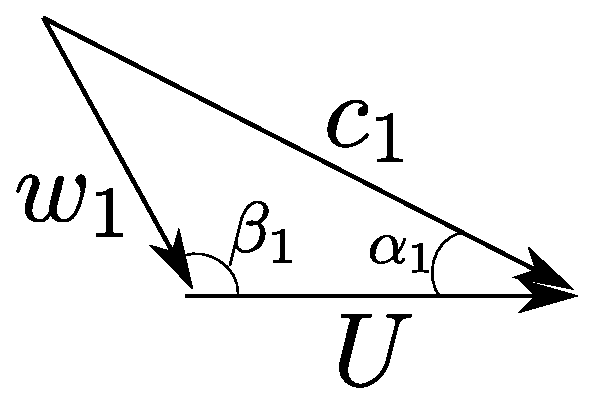
\includegraphics[height=2\fontcharht\font`\B]{triangulo.eps}%
  \endgroup
}
\begin{formuleo}[Fundamentalismos]
Euler:  $-\frac{\dot{W}}{\dot{m}}=\tau\cdot \Omega=-e=U_{2} \ctan{2}-U_{1} \ctan{1} =\left(h_{02}-h_{01}\right)=\left(\frac{c_{2}^{2}-c_{1}^{2}}{2}\right)+\left(\frac{U_{2}^{2}-U_{1}^{2}}{2}\right)+\left(\frac{w_{1}^{2}-w_{2}^{2}}{2}\right)$    \\
Primera Ley: $ \dot{U}=\dot{Q}-\dot{W} - \dot{m}\left[\left(h_{2}-h_{1}\right)+\frac{1}{2}\left(c_{2}^{2}-c_{1}^{2}\right)+g\left(z_{2}-z_{1}\right)\right]$
Rend. de la instalación: $\frac{\text{Potencia efectiva}}{\text{Potencia entregada a la instalación}}$    \\
\textbf{Ley de Coseno:} $c^2 = a^2+b^2 - 2ab\cos{\theta_{\widehat{ab}}}$
\end{formuleo}


\formuleoseparator


\begin{formuleo}[T. Hidráulicas]
Pelton: aprox Dixon $w_2\approx U\rightarrow$ $c_2 \approx 2 U \sin \frac{\beta_2}{2}$ donde $\beta_{2}=180^\circ-\vartheta_{2}$ \ $\eta_{\mathrm{h}}^{\mathrm{pelton}}=\frac{U\left(c_{1}-c_{\theta 2}\right)}{g H}$    \\
Kaplan: $\cax{1}=\cax{2} = \frac{Q}{\pi(r_{\mathrm{ext}}^2-r_{\mathrm{int}}^2)}$ \separar $\eta_{\mathrm{h}}^{\mathrm{kaplan}} = \frac{\dW/\dm}{gH}$    \\
$\text{Eficiencia Hidráulica} = \fractt{Potencia entregada al rotor}{Potencia que se puede entregar a la instalación (potencial)}$
\end{formuleo}


\formuleoseparator


\begin{formuleo}[T. de Vapor]
Trabajo: $\mathrm{d} e=\frac{1}{\rho} \mathrm{d} p+\mathrm{d} \frac{1}{2} c^{2}+\mathrm{d} q$\separar
Tobera: $\eta_{\mathrm{iso}}^{\mathrm{tobera}}=\frac{c_{1}^{2} / 2}{c_{1 s}^{2} / 2}$; $K_{f}=\frac{c_{1}}{c_{1 s}}$ \separar 
Rotor: $dp=0:\ \eta_{\mathrm{iso}}^{\mathrm{rotor}}=\frac{\dot{W} / \dot{m}}{c_{1}^{2} / 2}$ con $K_{m}=\frac{w_{2}}{w_{1}}$ \separar Eficiencia interna de etapa: $\eta_{i}=\eta_{\mathrm{iso}}^{\mathrm{tobera}} \cdot \eta_{\mathrm{liso}}^{\mathrm{rotor}} \cdot \ldots=\frac{\dW / \dot{m}}{\Delta h_{s}}$ Eficiencia maxima: $\frac{U}{c_{1}}=\frac{\cos \alpha_{1}}{2m \cdot(1-\degreeofreaction)} $ \\ 
\textbf{Escalonamiento de reacción}. Fijo: $c_{2s}=\sqrt{2 \Delta h_{s}(1-\degreeofreaction )+c_{1}^{2}}$  Movil: $w_{2s}=\sqrt{2 \Delta h_{s}\degreeofreaction +
w_{1}^{2}}$ donde $K_m = \frac{w_2}{w_{2s}}$\\ Perdidas tobera: $Y_{\mathrm{tob.}}=\dot{m}(c^2_{1s}/2-c^2_1/2)$  Perdidas movil: $Y_{\mathrm{m}} = \dot{m}(w_1^2/2 - w_2^2/2)$
Perdidas roz. entre fijo/movil: $k_{\mathrm{axial}}=0,009$ ,$k_{\mathrm{radial}}=0,027$ : $Y_{\mathrm{roz.}}=k \rho n_{\mathrm{Hz}}^{3} D_m^{5}$ [W]\separar Perdidas ventil. $\varepsilon$ es grado adm. $l$ es largo alabes en \emph{cm}, $D_m$ es diametro medio y $k$ depende del nro. de ruedas $k_1=3,8$; $k_2=4,5$; $k_3=6 \going $ $Y_{\mathrm{vent.}}=(1-\varepsilon) k \rho n^{3} D_m^{4} l$ [W].  donde $\varepsilon = \fractt{Long arco inyeccion}{circunferencia media (U/omega)}$ donde $\ell_a = \frac{\dm}{\rho h c_0}$ para una ÚNICA tobera cuadrada $A=\ell_a \cdot h$  \\
Etapa acción: $c_0\approx 0$ para tobera. Rend. Maximo de UNA etapa accion ($c_1$ salida tobera): $\eta_{\max} = \frac{\dW/\dm}{c_{1s}^2/2}= K_f^2 \cdot \frac{\cos^2(\alpha_1)}{2}\cdot (1+K_m \frac{\cos \beta_1}{\cos \beta_2})$
\end{formuleo}


\formuleoseparator


\begin{formuleo}[T.Gas]
Valores: ${\cp}_{comb} \approx 1,15$ [kJ/kg]; $\ctegas_{comb.} \approx 1,33$; $\eta_{\mathrm{comb}} = \frac{\operatorname{FAC}_t}{\operatorname{FAC}_c}$

Relacion de compresion (Segun Hilal): $\relcomp = \frac{p_2}{p_1}$  Potencia eff donde $w=\Delta h$    \\
$\dot{W}_{e}=\left(\dot{m}_{\mathrm{air}}+\dot{m}_{\mathrm{comb.}}\right) \cdot |w_{\mathrm{turb.}}|-\dot{m}_{\mathrm{air}} \cdot |w_{\mathrm{comp.}}|$ donde $w_t = h_{\mathrm{in}}-h_{\mathrm{out}}={\cp}_{\mathrm{cte}} (T_{\mathrm{in}}-T_{\mathrm{out}}) $ \\
Eficiencias Internas: $\etaint^{\mathrm{turb.}} = \fractt{Potencia ciclo indicado}{Potencia ciclo ideal} = \frac{\Delta h}{\Delta h_s}$     Efic. mecánicas(al reves para bombas): $\etamec^{\mathrm{turb.}} = \fractt{Potencia entregada}{Potencia indicada} = \frac{w_t}{w^{\mathrm{ind}}_{t}} $    \\
Optimo $\rTc$: $\relcomp^* =\left(\frac{T_{3}}{T_{1}} \eta_{c} \eta_{t} \frac{c_{34}}{c_{12}}\right)^{\left(\frac{\ctegas}{2(\ctegas-1)}\right)}$
Regeneración: $\sigma=\frac{T_A-T_2}{T_4 - T_2}$,$\rTc = \frac{T_2}{T_1}$,$\rTt=\frac{T_3}{T_1}$,$\eta_{\mathrm{regen}} = \frac{\rTc  -1}{\rTc} \frac{\rTt-\rTc}{\rTt -\rTc - \sigma \frac{\rTt - \rTc^2}{\rTc}} $ 
\separar Poder Calorico del combustible (PCI) [J/kg] Consumo especifico $\Ce = \frac{\dot{m}_{\mathrm{comb.}}}{P_e}\going$ $\eta_{\mathrm{instalacion}} = \frac{\dW_e}{\dot{m}_{\mathrm{comb.}} \cdot \mathrm{PCI}}=\frac{1}{\Ce \cdot\mathrm{PCI}}$   \\

\end{formuleo}


\formuleoseparator


\begin{formuleo}[Ciclo combinado]
Rankine: $\eta=\frac{\dot{W}_{\mathrm{t}} / \dot{m}-\dot{W}_{\mathrm{b}} / \dot{m}}{\dot{Q}_{\mathrm{in}} / \dot{m}}=\frac{\left|\Delta h_{\mathrm{turb} .}\right|-\Delta h_{\mathrm{bomba}}}{\Delta h_{\mathrm{cald}}}=1-\frac{\left|\Delta h_{\mathrm{cond} .}\right|}{\Delta h_{\mathrm{cald}}}$\separar $\mathrm{BWR}=\frac{\dot{W}_{\mathrm{b}} / \dot{m}}{\dot{W}_{\mathrm{t}} / \dot{m}}=\frac{\Delta h_{\mathrm{bomba}}}{ | \Delta h_{\mathrm{turb}} |}$ \separar Turb/bomba ($b$ al revés): $\eta_{\mathrm{t}}=\frac{\Delta h_{\text { turb }}}{\left(\Delta h_{\text { turb. }}\right)_{s}}$
\veltriangle
\end{formuleo}
\formuleoseparator

% Cosas que faltaron: Brayton formas de aumentar potencia/rendimiento y como influia cada una la potencia/rendimiento

%




\end{document}